\section{Process}
\subsection{Overall Roadmap}

In order to obtain a smaller model, less training and running with better performance,
we decided to make multiple models and training improvements based on DCGAN\upcite{dcgan} and improved it through multiple sets of experiment.
Figure \ref{roadmap} is the overall technical roadmap of this study.

\begin{figure}
    \begin{center}
    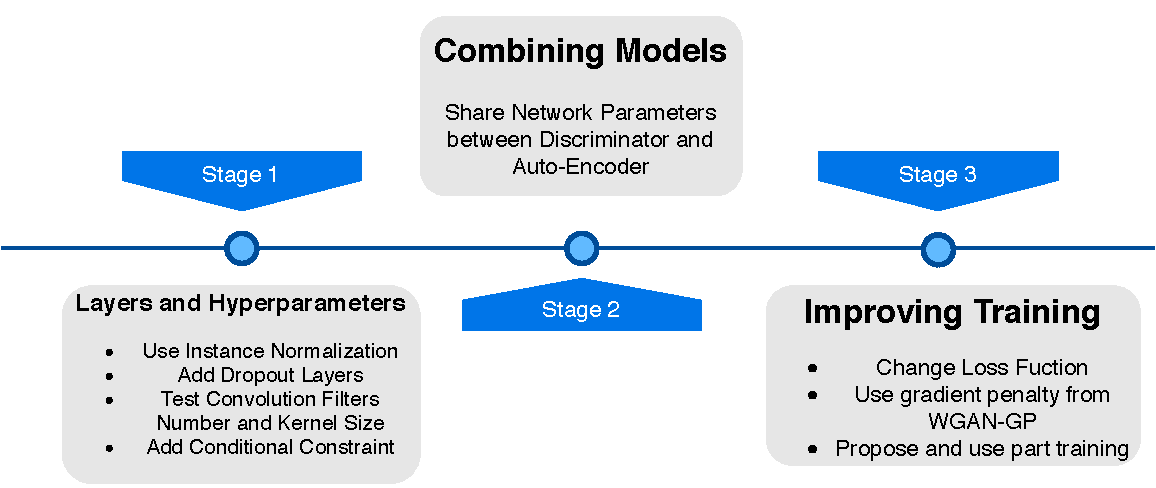
\includegraphics[width=\textwidth]{figures/roadmap.pdf}
    \caption{Overall technical Roadmap}
    \label{roadmap}
    \end{center}
\end{figure}


\subsection{Research Process}

In previous model adjustments, we conducted several comparative tests to select suitable hyperparameters.

Figure \ref{norm_bach} and Figure \ref{norm_instance} show the results of model after training 2 epochs using batch normalization and instance normalization respectively (about 5500 iterations per epoch).
It can be seen that the image quality is improved under the same training amount after using instance normalization,
    which means that the convergence speed of the model is faster.

\begin{figure}
    \begin{minipage}[t]{0.48\linewidth}
        \centering
        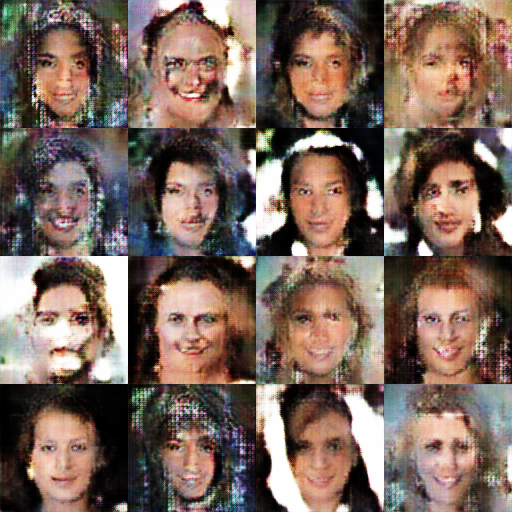
\includegraphics[width=\textwidth]{figures/result_norm_batch.png}
        \caption{Test result using Batch Normalization after training 2 epochs}
        \label{norm_bach}
    \end{minipage}
        \hfill
    \begin{minipage}[t]{0.48\linewidth}
        \centering
        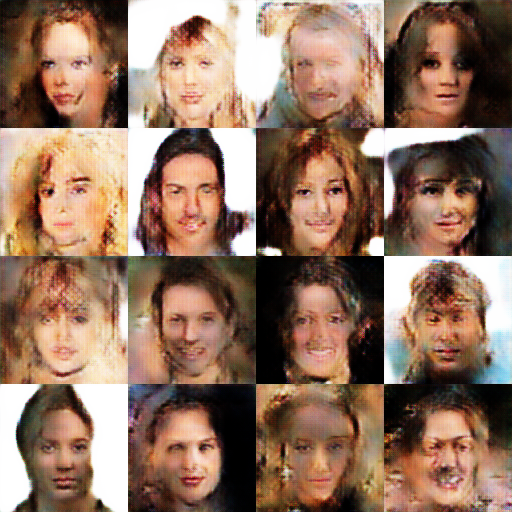
\includegraphics[width=\textwidth]{figures/result_norm_instance.png}
        \caption{Test result using Instance Normalization after training 2 epochs}
        \label{norm_instance}
    \end{minipage}
\end{figure}

In addition, we tested the effects of convolution kernel size and numbers of convolution filters on model performance and model size.
Fig.\ref{conv_filter_16}, Fig.\ref{conv_filter_24}, and Fig.\ref{conv_filter_32} are convolution filters using 16 times, 24 times, and 32 times,
    respectively and the output results are completed after training 15 epochs.
Times of convolution filters mean the start amount of convolution kernel.
It will be doubled in each next layer of decoder and encoder.
It can be seen that after the convolution filters is lowered,
    the image quality does not decrease markedly under the same training amount.
In order to reduce the size of the model to achieve the purpose of reducing use-cost,
    we finally chose a 16 times convolution filters.

\begin{figure}
    \begin{minipage}[t]{0.48\linewidth}
        \centering
        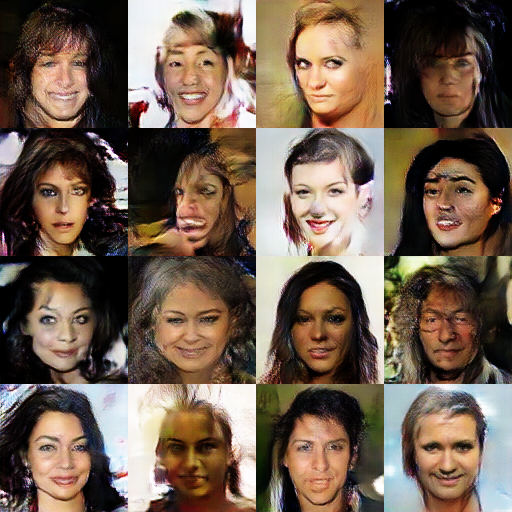
\includegraphics[width=\textwidth]{figures/result_conv_filter_16.png}
        \caption{Test result using 16x convolution filter after training 15 epochs}
        \label{conv_filter_16}
    \end{minipage}
        \hfill
    \begin{minipage}[t]{0.48\linewidth}
        \centering
        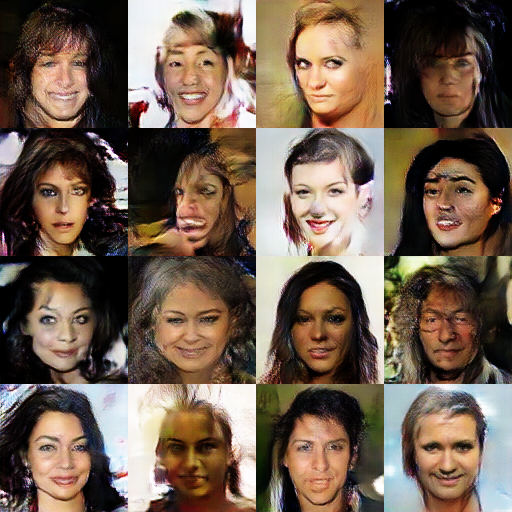
\includegraphics[width=\textwidth]{figures/result_conv_filter_24.png}
        \caption{Test result using 24x convolution filter after training 15 epochs}
        \label{conv_filter_24}
    \end{minipage}
    \begin{minipage}[t]{\linewidth}
        \centering
        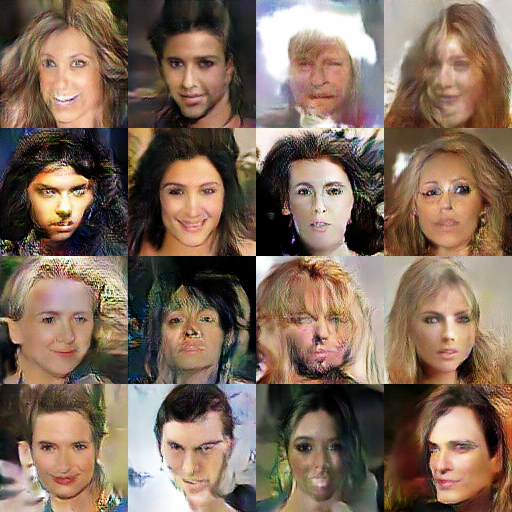
\includegraphics[width=0.48\textwidth]{figures/result_conv_filter_32.png}
        \caption{Test result using 32x convolution filter after training 15 epochs}
        \label{conv_filter_32}
    \end{minipage}
\end{figure}

Figure \ref{conv_kernel_5} and \ref{conv_kernel_3} show the results after training 4 epochs of the 5×5 and 3×3 (transposed) convolution kernel,
    respectively, under a 16 times convolution filter.
It can be seen that switching from a 5×5 convolution kernel to a 3×3 size,
    the image quality is degraded within an acceptable range, so we choose a 3×3 convolution kernel.

\begin{figure}
    \begin{minipage}[t]{0.48\linewidth}
        \centering
        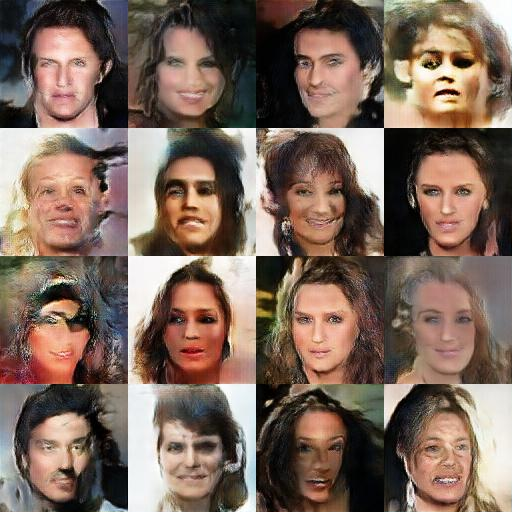
\includegraphics[width=\textwidth]{figures/result_conv_kernel_5.png}
        \caption{Test result using 5×5 convolution kernel after training 4 epochs}
        \label{conv_kernel_5}
    \end{minipage}
        \hfill
    \begin{minipage}[t]{0.48\linewidth}
        \centering
        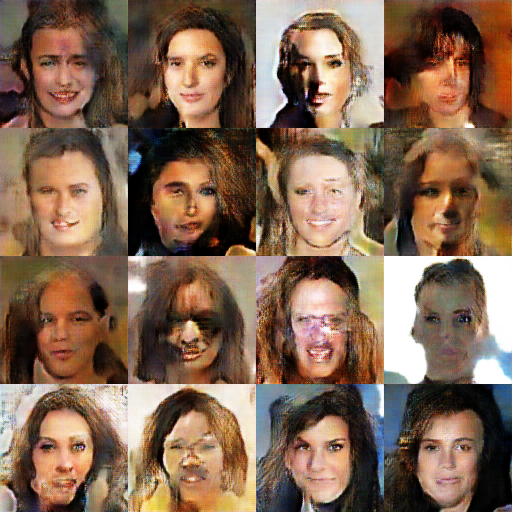
\includegraphics[width=\textwidth]{figures/result_conv_kernel_3.png}
        \caption{Test result using 3×3 convolution kernel after training 4 epochs}
        \label{conv_kernel_3}
    \end{minipage}
\end{figure}


\subsection{Model Overview}

After the research above, we finally obtained the conditional facial image generation and adjustment model.
It is as shown in Figure \ref{smliegan}.

\begin{figure}
    \begin{center}
    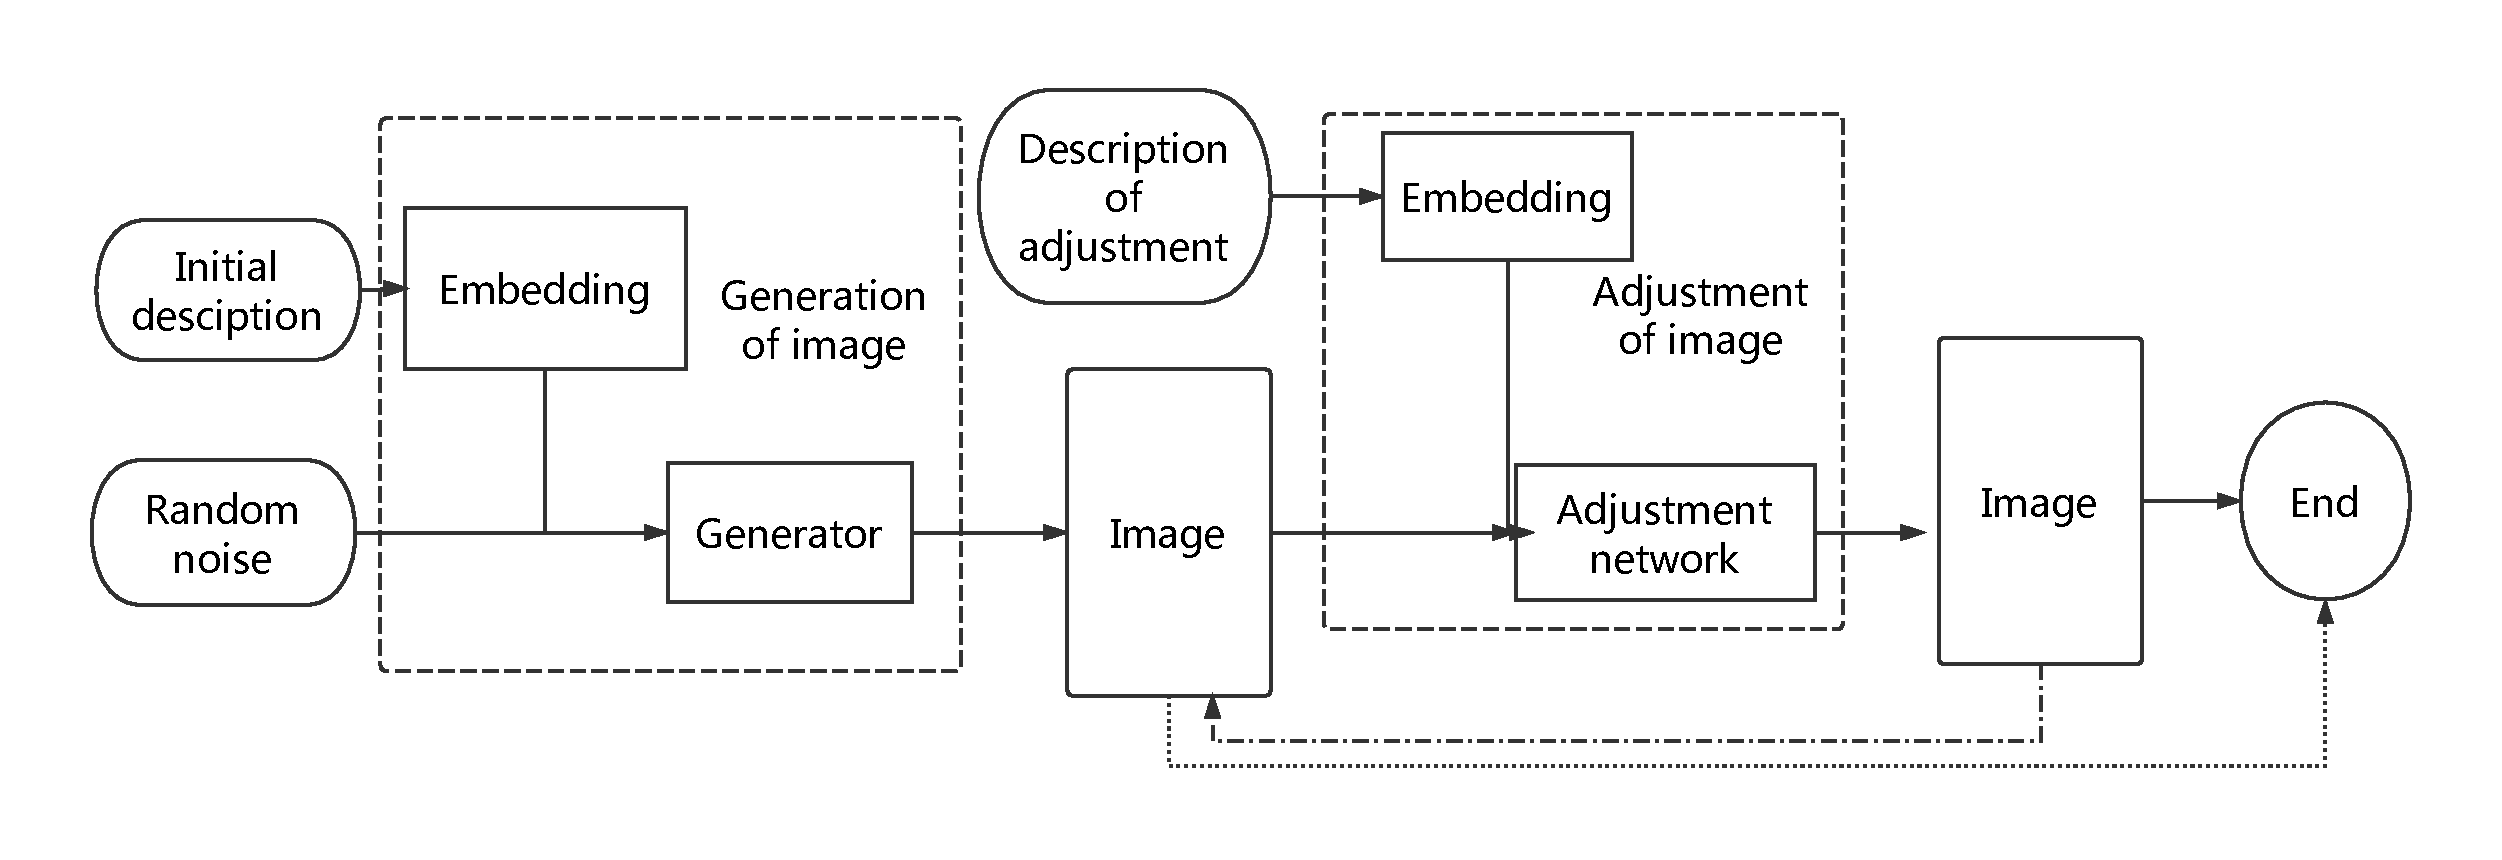
\includegraphics[width=\textwidth]{figures/model.pdf}
    \caption{The Model of LittleGAN}
    \label{smliegan}
    \end{center}
\end{figure}

LittleGAN consists of 3 networks and 2 main components.
The newtworks are generator, discriminator and adjustor.
The main components are encoder and decoder.
In LittleGAN, generator generates facial images from noise and facial attributes,
    and then adjustor combines it with new attributes to obtain new images.


\subsection{Decoder and Encoder}

Main components, encoder and decoder, are used for conversion of feature map and images.

An encoder can extract features from the image from global to local.
Using convolution, starting from an image of 128×128×3 (height × width × channels),
    the convolution with stride is continuously performed.
After each convolution, normalization, activation, dropout\upcite{dropout} is used.

The convolution layer uses a 5×5 convolution kernel.
Convolution filter is 16 in the first layer, doubled in each next layer.
So the image dimension is reduced when the feature is extracted.
    Also, the network has lower calculation amount.
Since we use gradient penalty\upcite{wgan-gp} in training,
    Instance Normalization\upcite{instance} is used at the same time.
To preserve the image for more information, Leaky ReLU (alpha=0.2) is used as the activation function.
In order to prevent occurrence of over-fitting,
    dropout\upcite{dropout} is used in the training to randomly hide some neurons to reduce the interaction between filters.

Decoder is used to generate an image from the feature map.
Using transposition convolution, the same number of filters,
    stride and convolution kernel are symmetrically used with the encoder.
Normalization and activation are performed after each transposition convolution as the same as the encoder.

%todo continue
\subsection{Generator and Discriminator}

We also named the combination of discriminator and generator as GAN network.
Generator consists of a fully connected layer and a decoder.
The facial attributes are combined with latent maps (conform to the normal distribution) as input to generate images by generator.
Discriminator consists of an encoder and 2 fully connected layers.
It uses images as input then extracts features and the probability of image comes from data.


In generator, through a fully connected layer, the input is combined and transformed into feature map(in 4×4×16n size).
Then the image is generated from global to local by decoder layers.
Finally a 3 filters convolution without stride is performed and used.
The tanh function is activated to obtain a three-channel (RGB) color image of 128×128×3 size.
Figure \ref{net_generator} is the graph of generate network structure.

\begin{figure}
    \begin{minipage}[t]{0.48\linewidth}
        \centering
        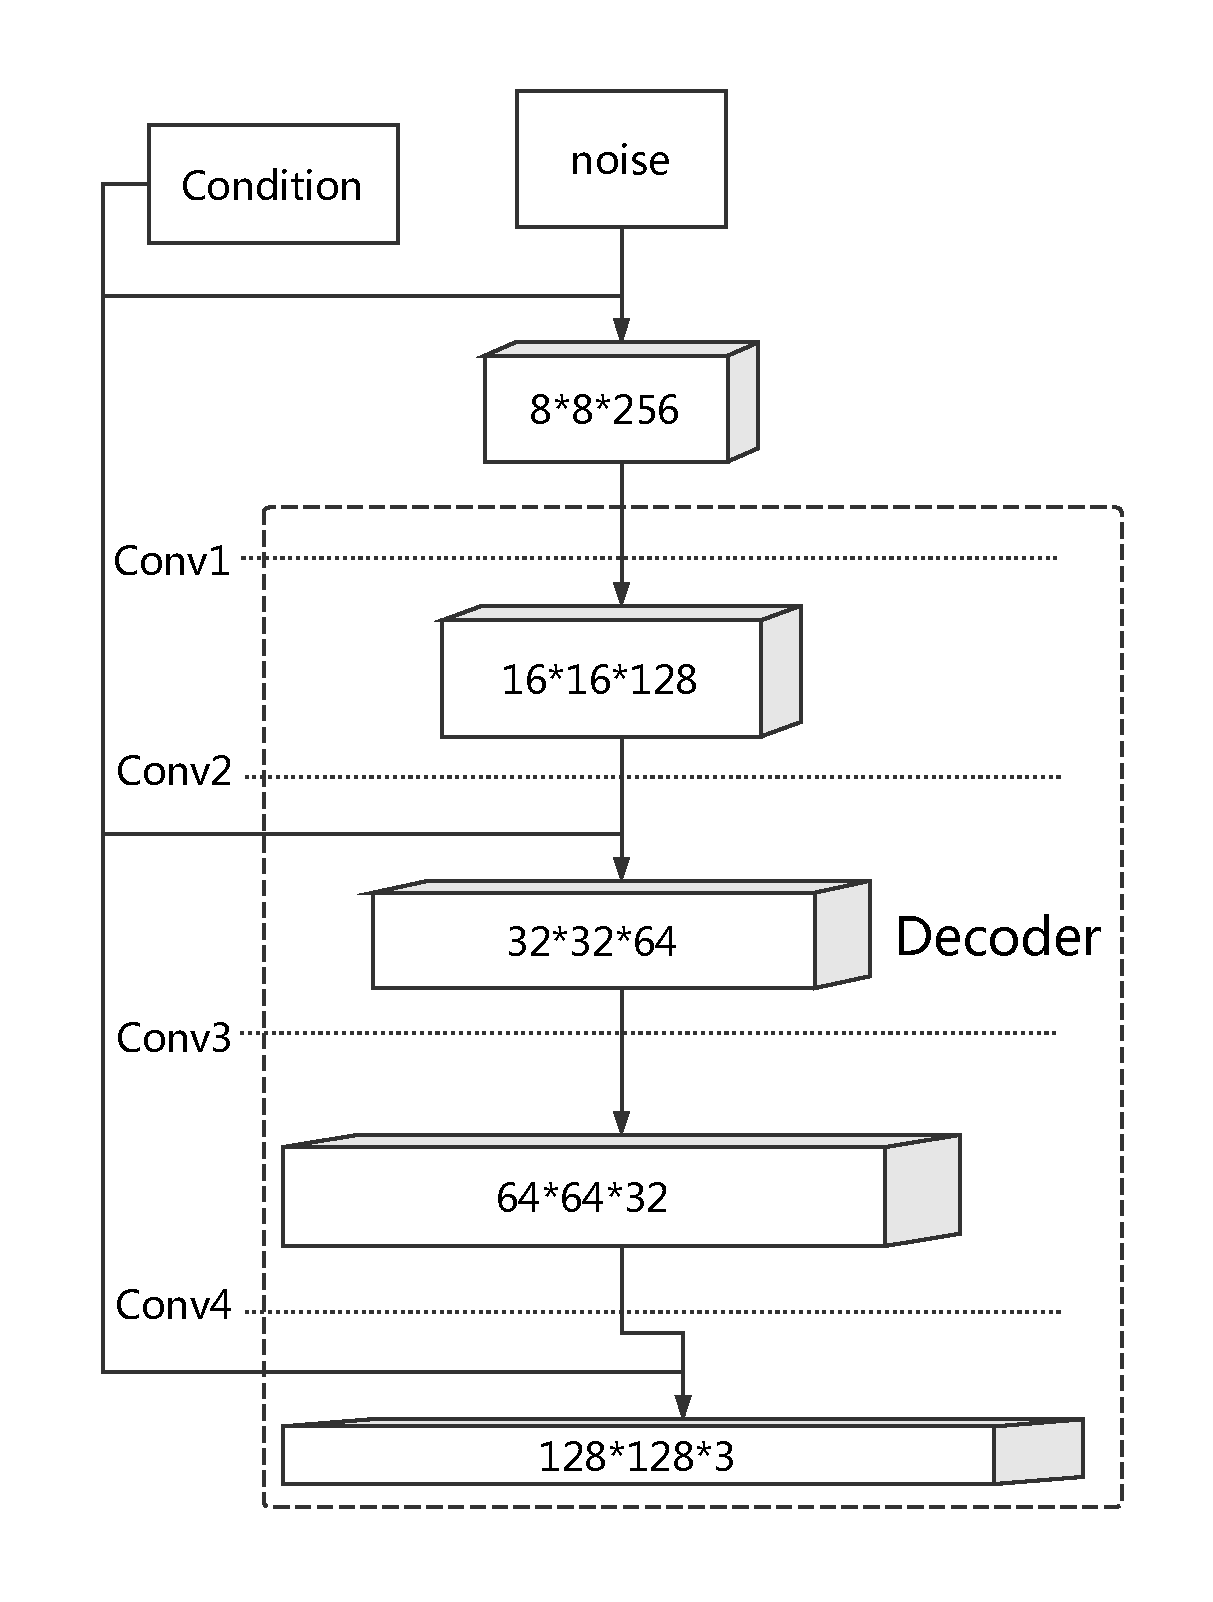
\includegraphics[width=\textwidth]{figures/net_generator.pdf}
        \caption{Generator Network Structure of LittleGAN}
        \label{net_generator}
    \end{minipage}
        \hfill
    \begin{minipage}[t]{0.48\linewidth}
        \centering
        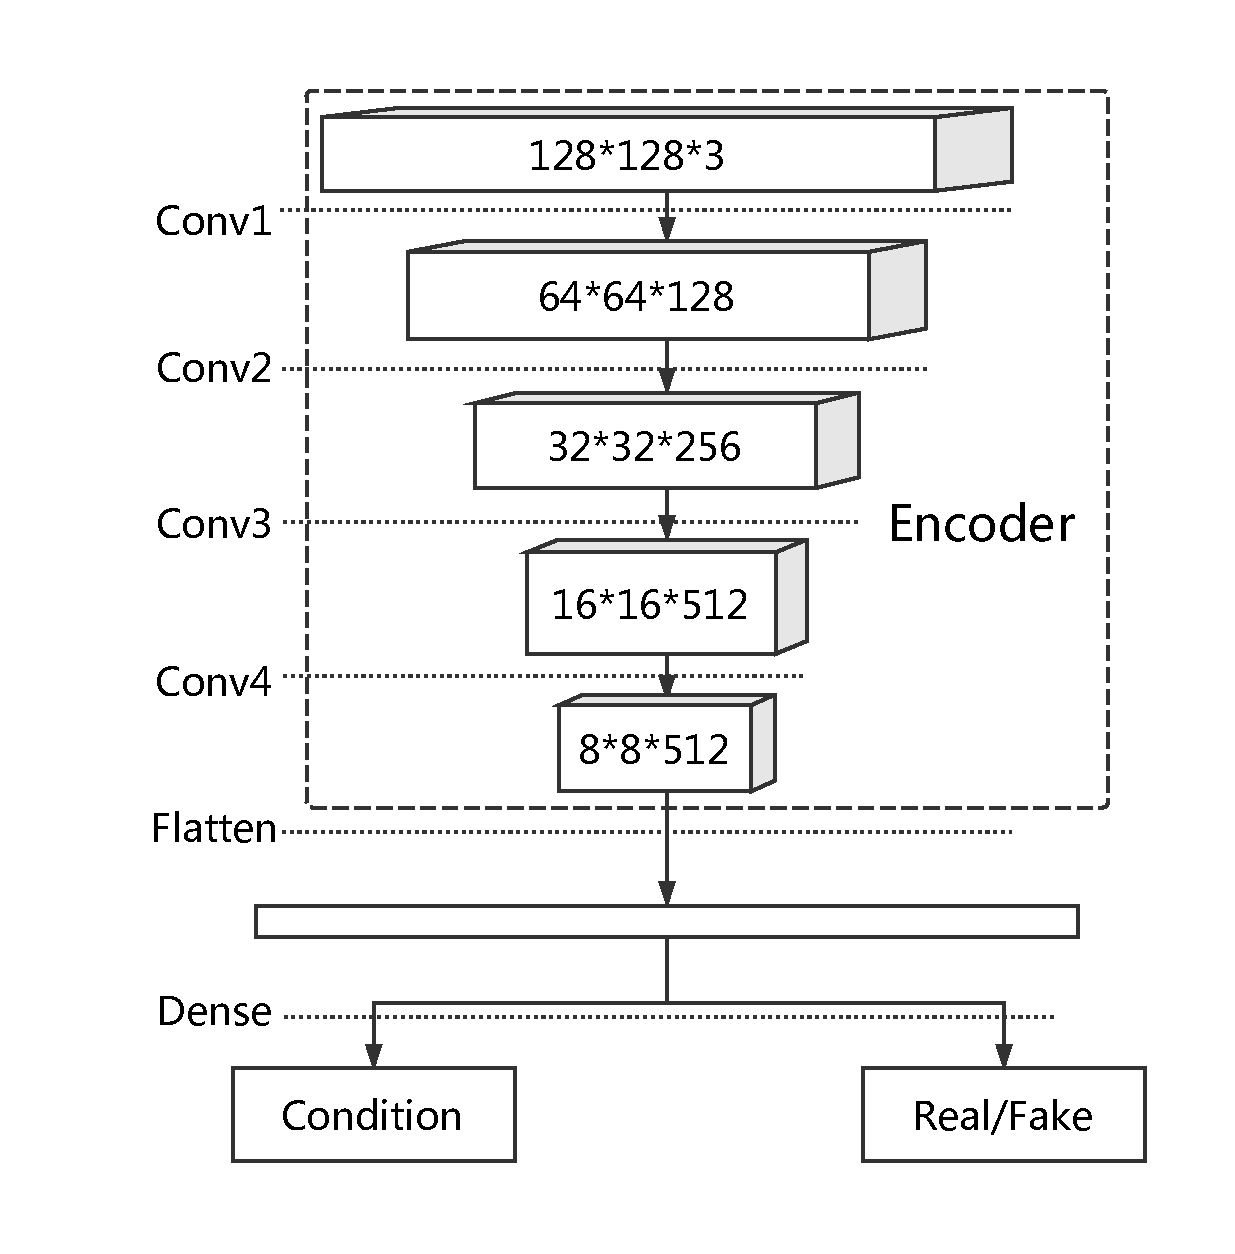
\includegraphics[width=\textwidth]{figures/net_discriminator.pdf}
        \caption{Discriminator Network Structure of LittleGAN}
        \label{net_discriminator}
    \end{minipage}
\end{figure}

Discriminator use encoder to extracts the feature map from the input image first.
Then on the one hand, the feature map is connected to the dimension 1 through a fully connected layer.
The Sigmoid activation function is used to normalize the result to [0,1],
    which indicates the possibility that the image comes from real data.
On the other hand, feature map is connected to the same dimension as attribute,
    the latent facial attribute information is extracted,
    and the result is also normalized to [0,1] using the Sigmoid activation function,
    thereby indicating the possibility that the image has these facial attributes.
Figure \ref{net_discriminator} is the graph of generate network structure.


For discriminator loss function, since the Sigmoid is used to activate the output,
    in order to ensure that the network parameters will not dead,
    we expect the loss of discriminator output to [0.02,0.98] instead of [0,1].
Since discriminator not only outputs probability of image comes from data but also contains the facial attribute information implied by the image,
    its loss includes the GAN loss and the conditional judgment loss.
In discriminator, we expect the output from real image close to 0.98, while the output from fake image close to 0.02.
Similarly, we expect the facial attribute information output by discriminator is as consistent as possible with the real data.
Equation \eqref{loss_d_gan}, Equation \eqref{loss_d_c}, and Equation \eqref{loss_d} are the GAN loss,
    conditional adjustment loss and total loss of discriminator, respectively.

% Todo: Add comment for equation
\begin{equation}
    Loss_{D-GAN}(D,G)=
    \mathbb{E}_{y\thicksim P(data)}[(0.98-D(y))^2]+
    \mathbb{E}_{c,z\thicksim P(fake)}[D(G(c,z)-0.02)^2]
    \label{loss_d_gan}
\end{equation}


\begin{equation}
    Loss_{C}(C)=
    \mathbb{E}_{c,y\thicksim P(data)}[(c-C(y))^2]
    \label{loss_d_c}
\end{equation}

\begin{equation}
    Loss_{D}(C,D,G)=
    Loss_{D-GAN}(D,G)+
    Loss_{C}(C)
    \label{loss_d}
\end{equation}

We add a mean absolute error to generator's loss function.
We expect overall color and layout to be more realistic while keeping the diversity generation results in this way.
The target of generator is to generate an image that treat the discriminator think it's from real data,
    and let discriminator output the attribute close to generation condition.
Therefore, the loss function of generator include into discriminator loss and the mean absolute error loss.
Equation \eqref{loss_g_gan}, Equation \eqref{loss_g_l1}, and Equation \eqref{loss_g} are the discriminator loss,
    mean absolute error loss and total loss of generator, respectively.
The $\lambda$ in the total loss in the experiment is 0.02.

\begin{equation}
    Loss_{G-GAN}(C,D,G)=
    \mathbb{E}_{c,z\thicksim P(fake)}[(0.98-D(G(c,z)))^2]+
    \mathbb{E}_{c,z\thicksim P(fake)}[(c-C(G(c,z)))^2]
    \label{loss_g_gan}
\end{equation}

\begin{equation}
    Loss_{G-L1}(G)=
    \mathbb{E}_{c,y,z\thicksim P(data)}[|y-G(c,z)|]
    \label{loss_g_l1}
\end{equation}

\begin{equation}
    Loss_{G}(C,D,G)=
    Loss_{G-GAN}(C,D,G)+
    \lambda Loss_{G-L1}(G)
    \label{loss_g}
\end{equation}

Our goal is to minimize the loss function of generator and discriminator,
    so the optimization goal of generator against the network is Equation \eqref{gan_target}

\begin{equation}
    GAN^*=\arg \min_{C,D} \max_{G}Loss_{D}(C,D,G)+Loss_{G}(C,D,G)
    \label{gan_target}
\end{equation}


\subsection{Adjustor Network}
Adjustor consists of a decoder, an encoder, several shortcut channels and a combined channel of adjustment conditions.
It uses an encoder to extract features from global to detail,
    and transmits each layer feature to the decoder network through a shortcut channel.
This makes each layer of the network does not need to carry all the information of the image.
Adjuster uses the decoder to combine the extracted features and adjustment conditions step by step to generate an image from detail to global.

Figure \ref{net_adjustor} is the graph of generate network structure.

\begin{figure}
    \begin{center}
    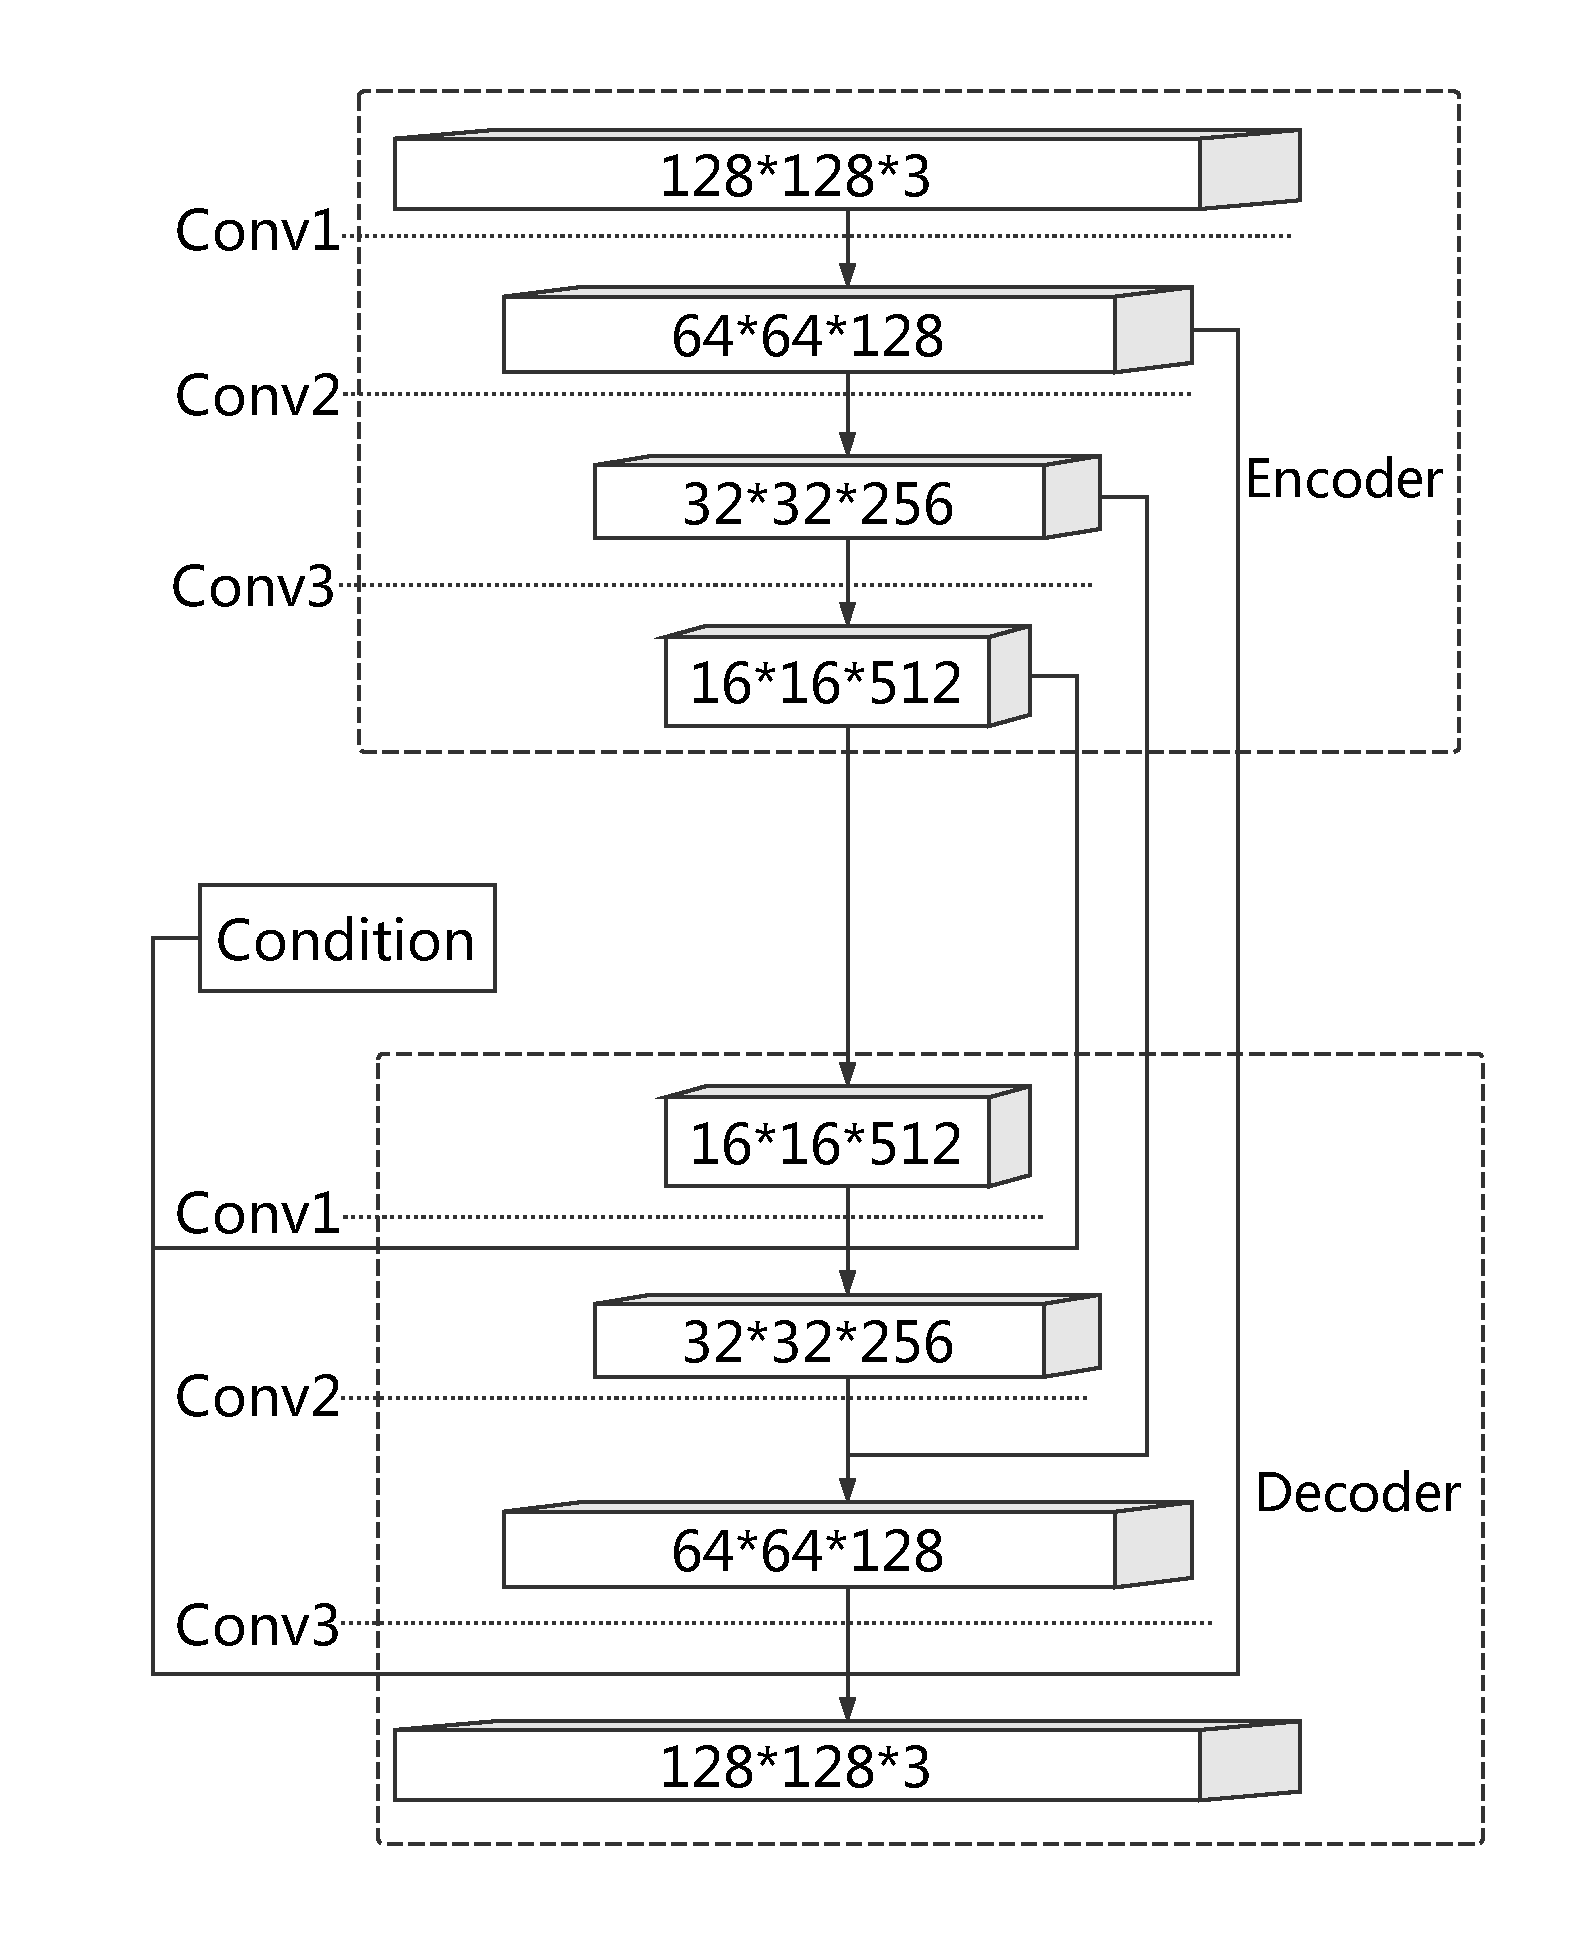
\includegraphics[width=0.48\textwidth]{figures/net_adjustor.pdf}
    \caption{Adjustor Network Structure of LittleGAN}
    \label{net_adjustor}
    \end{center}
\end{figure}

In adjustor network, the decoder and encoder parameters are shared with GAN's.
We use GAN loss and absolute mean error as a loss function for adjustor network.
Equation \eqref{loss_a_gan}, Equation \eqref{loss_a_l1}, and Equation \eqref{loss_u} are the GAN loss,
    mean absolute error loss and total loss of adjustor, respectively.

\begin{equation}
    Loss_{A-GAN}(C,D,A)=
    \mathbb{E}_{c,y\thicksim P(data)}[(0.98-D(A(c,y)))^2]+
    \mathbb{E}_{c,y\thicksim P(data)}[(c-C(A(c,z)))^2]
    \label{loss_a_gan}
\end{equation}

\begin{equation}
    Loss_{A-L1}(A)=
    \mathbb{E}_{c,x,y\thicksim P(data)}[|y-A(c,z)|]
    \label{loss_a_l1}
\end{equation}

\begin{equation}
    Loss_{A}(C,D,A)=
    Loss_{A-GAN}(C,D,A)+
    \lambda Loss_{A-L1}(A)
    \label{loss_u}
\end{equation}

\subsection{Model Training}
There are two main improvements to the training method of the model:
    applying the gradient penalty\upcite{wgan-gp} to discriminator,
    improving the convergence speed and the stability;
    using the partition training that proposed by us,
    enables the network to adjust the previous network layer more effectively,
    so that speed up the convergence.

The specific operation of the partition training proposed by us is as follows.
The network layer parameters that need to be trained in the model are grouped according to the function and the number of parameters.
When training each group of parameters,
    other parameters are fixed and only the parameters in the group are back-propagated.
In practice, for the overall effect of the model,
    we generally cross the overall model training and partition training in a certain proportion.
We set up separate optimizers for each set of parameters if use graph mode.
Although this will take up more memory for the training device,
    it can reduce the CPU's burden that the optimizer frequently switches the optimization target and reconstructs the model.